\tikzset{evalve/.style={draw, circle, inner sep=0pt, text width=3mm, align=center}}
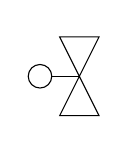
\begin{tikzpicture}
%elec-valve
\node(n1) at (4.25,2) {};
\node(n2) at (3.75,2) {};
\node(n3) at (4.25,1) {};
\node(n4) at (3.75,1) {};
\node(n5) at (4,1.5) {};
\node(n6) at (3.5,1.5) [evalve] {};
\draw(n1.center)--(n2.center)--(n3.center)--(n4.center)--(n1.center)--(n2.center);
\draw(n5.center)--(n6);
\addvmargin{4mm}
\end{tikzpicture}

    